% !TEX root = main.tex
% !TEX program = pdflatex


\section{Especificação e montagem do protótipo}
\label{sec:montagem}

Conforme mencionado nas seções anteriores, o robô construído possui três rodas em uma configuração simétrica. Apesar da falta de redundância -- pois se alguma das rodas falhar se perde a holonomicidade --, robôs omnidirecionais com 3 rodas (TOMR) são utilizados com mais frequência por serem mais simples de se implementar, apresentarem custo mais baixo (pois motores e rodas são responsáveis por 53\% do custo do projeto, conforme o \hyperref[sec:custo]{Apêndice A}), e uma certa economia de peso.
eird since it's a conversion from a regula
As rodas utilizadas -- mostradas na Figura \ref{fig:omniwheel} --, medem 58 mm de diâmetro, com estrutura em plástico e dez roletes emborrachados, e possuem capacidade de carga nominal de 3 kg \citep{omniwheel}, suficiente para os fins de demonstração do projeto. Cada roda é acionada por um motor de corrente contínua com caixa de redução, com uma velocidade nominal no eixo de saída de 210 rpm para uma tensão de 6 V. A máxima potência do motor está especificada para uma corrente de 1,1 A, a 110 rpm. Incluso no motor está um \textit{encoder} de quadratura, que permite a leitura da velocidade da roda e da direção de rotação. Com a relação de redução, se tem que para cada revolução da roda se tem 341,2 pulsos do sensor, e portanto cada pulso representa 0.01841 radianos \citep{motor}.
%Mais info sobre a ponte H: http://linksprite.com/wiki/index.php5?title=DC_Motor_Driver_Breakout_%28L298_Chipset%29#Arduino_Sample_Code

Além da utilização dos \textit{encoders} para implementação da odometria, também foi instalada na estrutura uma bússola, para garantir uma medida absoluta da orientação do robô (sem os erros que se acumulam nos métodos de \textit{dead-reckoning}). O modelo utilizado é a HMC5883L, já instalada em uma placa com alguns componentes necessários para seu funcionamento. A precisão do circuito, de acordo com o fabricante, é de 2 graus \citep{HMC5883L}. Para complementar a odometria, também foi instalada no robô uma unidade de medidas inerciais MPU6050, que possui acelerômetro e giroscópio em torno dos três eixos utilizados \citep{MPU6050}. Os sensores descritos neste parágrafo foram adquiridos e montados à estrutura, porém não foi realizada sua implementação. Os dois periféricos utilizam o protocolo de comunicação I2C \citep{semiconductors2000i2c}, também compatível com o computador utilizado.

Foi adquirida também uma bateria com capacidade de carga de 2000 mAh e 7,2 V de tensão nominal. Ligados à bateria, se tem 3 reguladores de tensão \textit{step down} MP2307, especificados para fornecer corrente constante de 3 A cada um, suportando picos de até 4 A \citep{MP2307}. A tensão de saída dos reguladores foi configurada em 5 V (para o computador), 3,3 V (para os \textit{encoders}) e 6 V (para os motores). A bússola e a IMU tem tensão de alimentação de 3,3 V, podendo ser ligadas ao mesmo regulador que os \textit{encoders} quando forem eventualmente integradas ao sistema. Como cada motor opera em geral com correntes abaixo de 1 A, o regulador utilizado é adequado, porém apresenta margens de capacidade consideravelmente pequenas.

O acionamento dos motores se dá por um circuito de pontes H. Há duas destas placas, e cada uma pode acionar dois motores. Assim, se tem a possibilidade de utilizar mais um motor em trabalhos futuros. Os \textit{driver} são desenvolvidos em torno do circuito L298N, que pode fornecer 4 A de corrente contínua distribuída entre as cargas \citep{L298N}. O chaveamento de cada canal dos \textit{drivers} é feito por meio de modulação de largura de pulso, fornecida pelo computador. Assim como os demais componentes, os \textit{drivers} foram fornecidos integrados a uma placa montada, com terminais para fixação de cabeamento e dissipadores de calor.

Todo o processamento é realizado por um \textbf{Raspberry Pi}, um \emph{single board computer}, que utiliza a arquitetura \acrshort{arm} em seu processador, ideal para dispositivos alimentados por baterias por consumir pouca energia e gerar pouco calor. O processador possui quatro núcleos, e um \emph{clock} de 1,2 GHz -- poder computacional equivalente há um computador de mesa comum. O \acrshort{rpi} utiliza um sistema operacional GNU/Linux, e \emph{software} deve ser desenvolvido para ser executado nesta plataforma. Há ainda 40 pinos de \acrshort{gpio} que podem ser utilizados para conectar sensores, atuadores e diversos componentes, e suporte nativo a \acrshort{i2c} \citep{upton2014raspberry}.

Para unir todos os componentes descritos, se projetou uma estrutura central, como um chassi. Tal estrutura pode ser vista na Figura \ref{fig:chassi}. No centro geométrico da estrutura e na periferia, próximo a uma das rodas, foram feitos dois orifícios que devem acomodar uma caneta hidrográfica cada. Assim, durante a fase de testes, se pode acompanhar graficamente a evolução cinemática do robô. Devido a localização central de uma das canetas, todos os componentes foram instalados na periferia da estrutura. Se tomou ainda o cuidado de instalar os CI de acelerômetro e giroscópio o mais próximo ao centro possível, para que as componentes de aceleração centrípeta dos movimentos com componentes de rotação não influenciassem em demasiado nos resultados. A IMU poderia ter sido colocada no centro geométrico, e este erro poderia ser introduzido no traço da caneta. No entanto, como a odometria e localização dependem muito mais dos sensores montados nos motores do que da IMU, se preferiu manter a caneta no centro, mantendo o MPU6050 o mais próximo possível. A bússola também foi montada relativamente próxima ao centro do robô, se tomando o cuidado de alinhar os eixos dos sistemas de coordenadas dos sensores com os do robô.

\begin{figure}[h]
  \centering
  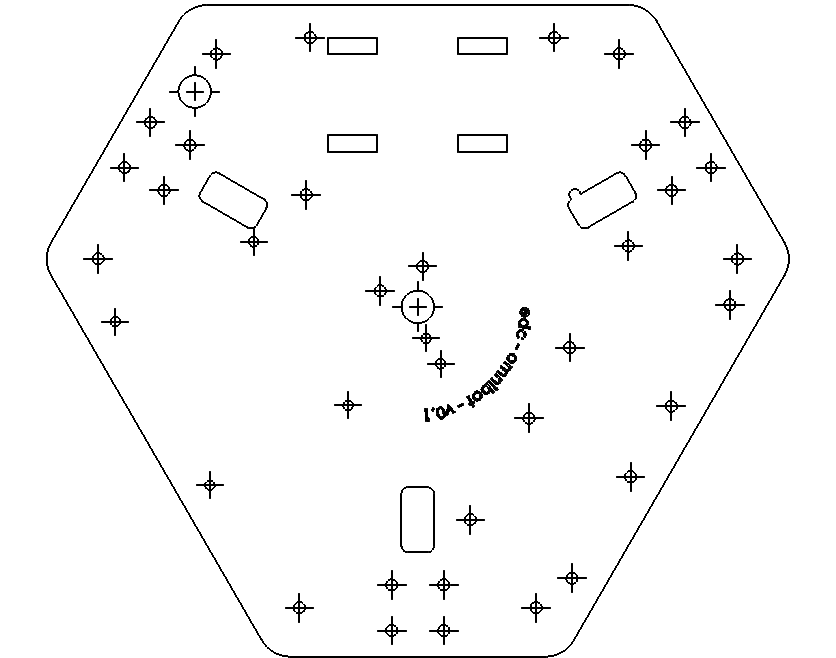
\includegraphics[width = 0.45\textwidth]{imagens/chassidxf}
  \caption{Chassi projetado.}
  \label{fig:chassi}
\end{figure}

Todos os componentes adquiridos possuem furos para fixação por meio de parafusos com 3 mm de diâmetro. A estrutura foi projetada com furos de 3,5 mm de diâmetro, para compensar possíveis erros de medição (visto que nem todos os componentes apresentaram seus desenhos nas informações técnicas) e possíveis tolerâncias de fabricação. Além dos furos de fixação dos componentes, também foram introduzidos orifícios próximos aos motores, para passagem dos cabos de um lado a outro da placa, e orifícios para fixação da bateria com presilhas plásticas. Na mesma área destinada à fixação da bateria se adicionou furação capaz de receber uma placa Arduino MEGA, caso se deseje utilizar um microcontrolador em trabalhos futuros. Também foram adicionados 6 furos na periferia do chassi, para possibilitar a montagem de outra chapa sobre a dos componentes, caso sejam realizados trabalhos que exijam a expansão da estrutura.

A plataforma projetada foi então fabricada, utilizando chapas de acrílico transparente de 5 mm de espessura. Se cogitou produzir tal estrutura em alumínio, porém se mostrou mais prático utilizar o acrílico. Entre as vantagens do material plástico se podem destacar a fácil obtenção, baixo custo, isolamento elétrico (permitindo montar os componentes eletrônicos diretamente sobre o chassi) e a possibilidade de fabricação utilizando uma máquina de corte a \textit{laser}, que elimina o limite inferior de tamanho de brocas e fresas em relação a fresadora CNC considerada originalmente. A espessura foi escolhida empiricamente, dentro das disponíveis, de maneira relativamente conservadora, e atendeu as necessidades. Na Figura \ref{fig:montagem} se pode ver a montagem final do protótipo. Os furos sobredimensionados não afetaram o alinhamento das peças.

\begin{figure}[h]
  \centering
  
\includegraphics[width = 0.45\textwidth]{imagens/edc}
  \caption{Protótipo montado, sem as canetas. TROCAR FIGURA}
  \label{fig:montagem}
\end{figure}

TERMINAR DE FALAR SOBRE AS LIGAÇÕES ELÉTRICAS QUANDO EU FIZER A LIGAÇÃO DEFINITIVA.
TERMINAR DE FALAR SOBRE AS LIGAÇÕES ELÉTRICAS QUANDO EU FIZER A LIGAÇÃO DEFINITIVA.
TERMINAR DE FALAR SOBRE AS LIGAÇÕES ELÉTRICAS QUANDO EU FIZER A LIGAÇÃO DEFINITIVA.
TERMINAR DE FALAR SOBRE AS LIGAÇÕES ELÉTRICAS QUANDO EU FIZER A LIGAÇÃO DEFINITIVA.

O custo de aquisição dos componentes relatados pode ser visto detalhado no \hyperref[sec:custo]{Apêndice A}. Cabe ressaltar que todos os itens foram comprados em dobro, para realizar a montagem de dois robôs para futuros trabalhos no LAMECC (Laboratório de Mecatrônia e Controle).

\section{Desenvolvimento Teórico}
\label{sec:teorico}

%% MODELAGEM:
%PARK: pg 468
\subsection{Modelagem Cinemática}

Primeiramente, se definem dois sistemas de coordenadas. O primeiro, $(x_I,y_I)$, é o sistema de coordenadas global, fixo no ambiente. O segundo, $(x_R,y_R)$, está centrado no próprio robô. Ainda se pode definir o ângulo $\theta$ como a orientação do robô -- ou seja, o ângulo entre os dois sistemas de coordenadas. Tal relação pode ser vista na Figura \ref{fig:ref}, e a transformação de um sistema para o outro é descrita na Equação \ref{eq:world_ref}, conforme \citet{siegwart2011introduction} e \citet{ritter2016modelagem}.

\begin{figure}[h]
  \centering
  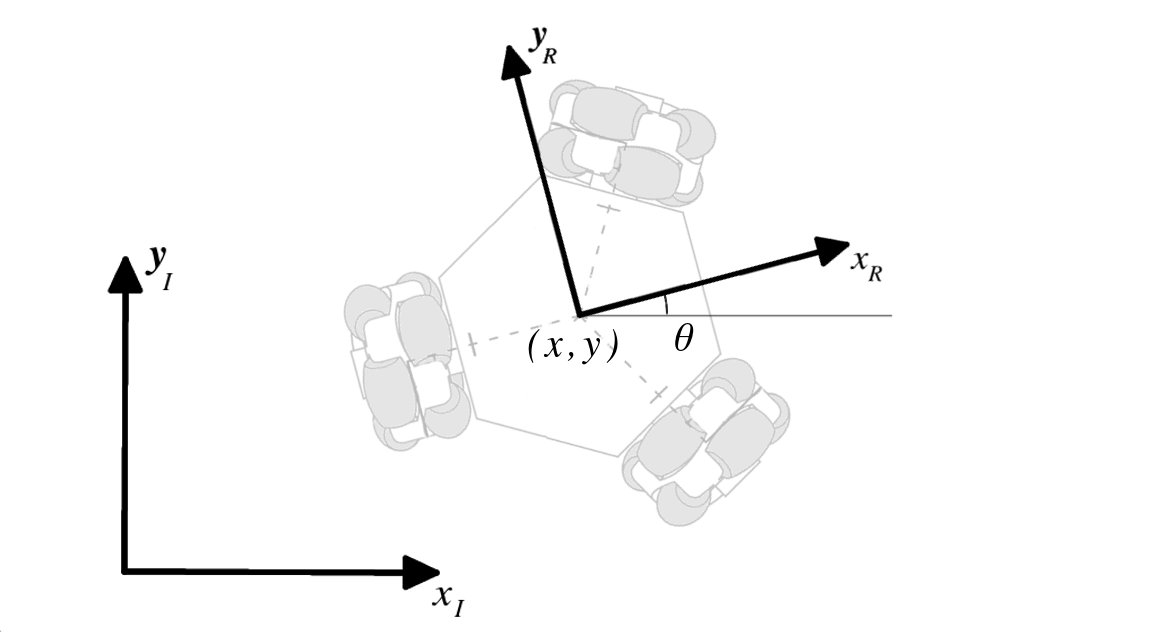
\includegraphics[width = 0.65\textwidth]{imagens/ref}
  \caption{Sistemas de coordenadas global I e relativo ao centro do robô R.}
  \source{Adaptado de \citet{ritter2016modelagem}}
  \label{fig:ref}
\end{figure}

\begin{equation}
  \begin{pmatrix}
    x_I \\
    y_I \\
    \theta
  \end{pmatrix}
  =
  \begin{pmatrix}
    cos \theta & -sen \theta & 0 \\
    sen\theta  &  cos \theta & 0 \\
    0          & 0          & 1
  \end{pmatrix}
  \begin{pmatrix}
    x_R \\
    y_R \\
    \theta
  \end{pmatrix}
  \label{eq:world_ref}
\end{equation}

O último termo da Equação \ref{eq:world_ref} também pode ser descrito como $q_R$, e o vetor de velocidades $[v_x, v_y, \omega_z]^T$, centrados no sistema de coordenadas do robô, é $\dot{q_R}$. Com o objetivo de mapear a velocidade de giro das rodas $\dot{\phi} = [\dot{\phi}_1, \dot{\phi}_2, \dot{\phi}_3]^T$ às velocidades $\dot{q_R}$, se utiliza a modelagem cinemática apresentada por \citet{siegwart2011introduction}, com as referências apresentadas na Figura \ref{fig:robo_vel}. Na figura,  A mesma modelagem é utilizada por \citet{ritter2016modelagem}, porém com outra sequência e sentido de giro para as rodas.

\begin{figure}[h]
  \centering
  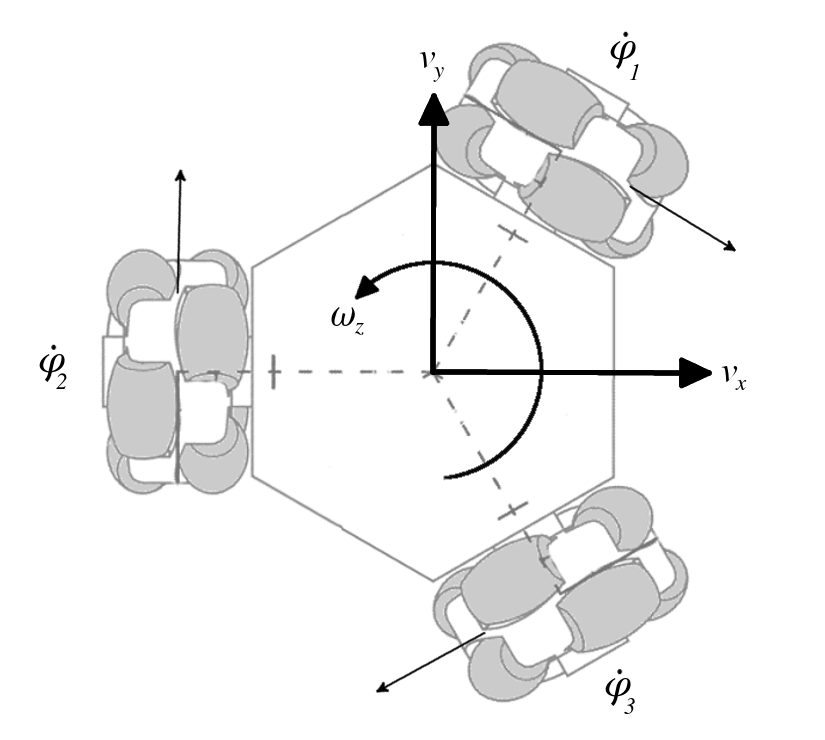
\includegraphics[width = 0.5\textwidth]{imagens/robot_vel4}
  \caption{Vista superior do robô, mostrando as convenções adotadas. As grandezas $v_x$ e $v_y$ estão no sistema de coordenadas do robô.}
  \label{fig:robo_vel}
\end{figure}

Assim, para um robô com 3 rodas dispostas em simetria radial em torno do centro da estrutura, a cinemática direta é dada pela Equação \ref{eq:dk}. Diversos autores utilizam variações da mesma modelagem (\citet{rojas2006holonomic}, \citet{pin1994new}, entre outros). Nas equações apresentadas, $r$ é o raio de cada roda e $R$ o raio do robô (a distância do centro da roda ao centro da estrutura do robô).

\begin{equation}
  \begin{pmatrix}
    v_x \\
    v_y \\
    \omega_z
  \end{pmatrix}
  =
  \frac{r}{3R}
  \begin{pmatrix}
    -\frac{3R}{\sqrt{3}} & 0   & \frac{3R}{\sqrt{3}} \\
    R                    & -2R & R                   \\
    1                    & 1   & 1
  \end{pmatrix}
  \begin{pmatrix}
    \dot{\phi_1} \\
    \dot{\phi_2} \\
    \dot{\phi_3}
  \end{pmatrix}.
  \label{eq:dk}
\end{equation}

Também se deseja utilizar a cinemática inversa do modelo, obtida realizando-se a inversão da matriz de transformação apresentada na Equação \ref{eq:dk}, é dada pela Equação \ref{eq:ik}. Nota-se que esta inversão é simplificada no caso do robô com 3 rodas, visto que quando há mais rodas é formada uma matriz $3 \times n$, sendo $n$ o número de rodas, e se deve utilizar uma matriz pseudo-inversa, conforme demonstrado por \citet{rojas2006holonomic}.

\begin{equation}
  \begin{pmatrix}
    \dot{\phi_1} \\
    \dot{\phi_2} \\
    \dot{\phi_3}
  \end{pmatrix}
  =
  \frac{1}{r}
  \begin{pmatrix}
    -\frac{\sqrt{3}}{2} & \frac{1}{2} & R \\
    0                   & -1          & R \\
    \frac{\sqrt{3}}{2}  & \frac{1}{2} & R
  \end{pmatrix}
  \begin{pmatrix}
    v_x \\
    v_y \\
    \omega_z
  \end{pmatrix}
  \label{eq:ik}
\end{equation}

Como pela classificação de \citet{campion1996structural} um \acrshort{tomr} é caracterizado na categoria (3,0), o modelo cinemático das equações \ref{eq:dk} e \ref{eq:ik} é controlável, estável e descreve a posição, orientação e suas derivadas de forma suficiente. % O modelo cinemático da Equação \ref{eq:dk} também é utilizado por \citet{rojas2006holonomic} e \citet{ritter2016modelagem}.

%% ODOMETRIA:
% lynch, pg 492 do pdf
\subsection{Odometria}

Durante a operação do robô, se torna necessário calcular a posição da estrutura. Para o cálculo da odometria, se utiliza a metodologia mostrada em \citet{lynch2017modern}. Se assume que durante um certo intervalo de tempo $\Delta t$ se tenha velocidades de rotação constantes nas rodas, o que permite considerar $\dot{\phi_i}.\Delta t = \Delta \phi_i$. Considera-se também que a unidade de tempo deste período é arbitrária, e como se deseja integrar no mesmo intervalo posteriormente, se assume um período unitário $\Delta t = 1$. Este procedimento está descrito na Equação \ref{eq:odo}, modificada a partir da Equação \ref{eq:dk}. Na prática, é fácil contar os deslocamentos angulares $\Delta \phi_i$, visto que o número de pulsos por revolução dos \textit{encoders} é determinado.

\begin{equation}
  \begin{pmatrix}
    v_x \\
    v_y \\
    \omega_z
  \end{pmatrix}
  =
  \frac{r}{3R}
  \begin{pmatrix}
    -\frac{3R}{\sqrt{3}} & 0   & \frac{3R}{\sqrt{3}} \\
    R                    & -2R & R                   \\
    1                    & 1   & 1
  \end{pmatrix}
  \begin{pmatrix}
    \Delta{\phi_1} \\
    \Delta{\phi_2} \\
    \Delta{\phi_3}
  \end{pmatrix}.
  \label{eq:odo}
\end{equation}

De posse das velocidades da plataforma durante o período de tempo unitário $\Delta t$ -- lembrando que $v_x$, $v_y$ e $\omega_z$ estão no sistema de coordenadas centrado no corpo do robô --, se deve avaliar o deslocamento em relação ao centro do robô na posição anterior. Para o caso em que $\omega_z = 0$, numa trajetória retilínea, se tem simplesmente que $\Delta q_R = \dot{q_R}$.

No entanto, quando houve mudança de orientação no período e consequentemente $\omega_z \neq 0$, se deve levar em consideração os desvios de trajetória causados por essa rotação. Assim, se obtem $\Delta q_R$ de acordo com a Equação \ref{eq:desvio} \citep{lynch2017modern}.

\begin{equation}
  \Delta q_R
  =
  \begin{pmatrix}
    \Delta x_R \\
    \Delta y_R \\
    \Delta\theta
  \end{pmatrix}
  =
  \begin{pmatrix}
    (v_x sen(\omega_z)) + v_y (cos(\omega_z) - 1)/\omega_z \\
    (v_y sen(\omega_z)) + v_x (1-cos(\omega_z)) / \omega_z \\
    \omega_z
  \end{pmatrix}
  \label{eq:desvio}
\end{equation}

Sendo $k$ o instante antes do período de tempo analisado, para se obter a nova posição $q_I$ do robô no sistema de coordenadas global se deve utilizar a rotação $R(\theta_k)$ apresentada na Equação \ref{eq:world_ref}, e atualizando os valores da última iteração conforme a Equação \ref{eq:new_odo}.

\begin{equation}
  q_{I(k+1)} = q_{I(k)} + \Delta q_I = q_{I(k)} + R(\theta_k) \Delta q_I
  \label{eq:new_odo}
\end{equation}
%\cite{samani2007comprehensive}: Adicionam um modelo de ruído dos encoders à estimativa. TIRAR OU ELABORAR?

%% PLANEJAMENTO DE TRAJETÓRIA:
\subsection{Planejamento de Trajetória}

Para o robô desenvolvido, não há a necessidade de implementar algoritmos complexos de planejamento de trajetória (detecção de obstáculos, caminhos de mínima energia, etc.). Serão abordados caminhos ``ponto a ponto'', que levam de um ponto inicial a um ponto final, ambos em repouso \citep{lynch2017modern}.

Apesar de ser uma trajetória simples, ainda se podem aplicar considerações para uma melhor operação do sistema. Uma dessas considerações é o chamado \textit{time-scaling} da trajetóra, ou seja, a geração de uma função $s(t)$ que suavize o comportamento do robô por meio de restrições em velocidades e acelerações. Na Figura \ref{fig:poly5} se pode ver uma curva de perfil de velocidade polinomial de quinta ordem, que pode garantir velocidades e acelerações nulas nos pontos de origem e destino.

\begin{figure}[h]
  \centering
  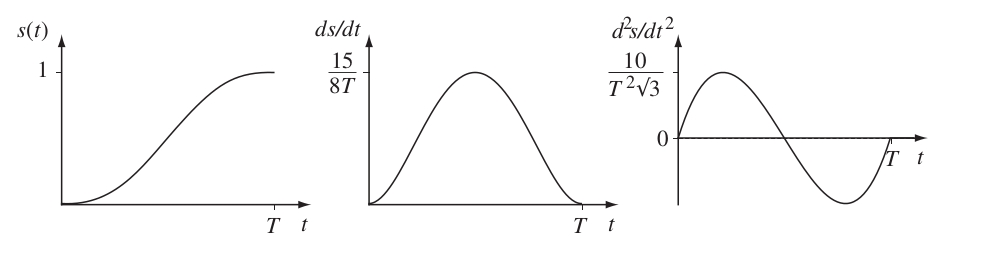
\includegraphics[width = 0.85\textwidth]{imagens/poly5}
  \caption{Deslocamento, velocidade e aceleração durante uma trajetória gerada por polinômio de quinta ordem. Aceleração e velocidade são nulas tanto no ponto de origem quanto no ponto de destino.}
  \source{\citet{lynch2017modern}}
  \label{fig:poly5}
\end{figure}

No entanto, a interpolação de um polinômio a cada cálculo de trajetória é um processo que pode envolver um certo custo computacional elevado, e devido à simplicidade dos componentes utilizados, se julgou que o aumento de suavidade na operação não fosse significativo. Portanto, neste trabalho se optou por utilizar um perfil de velocidade trapezoidal, conforme mostrado na Figura \ref{fig:trap}. Tal perfil é um dos mais comuns em robótica, devido a sua simples implementação. Os limites de aceleração foram definidos na fase de implantação do \textit{software}, de modo a evitar o deslizamento das rodas utilizadas na superfície de testes.

\begin{figure}[h]
  \centering
  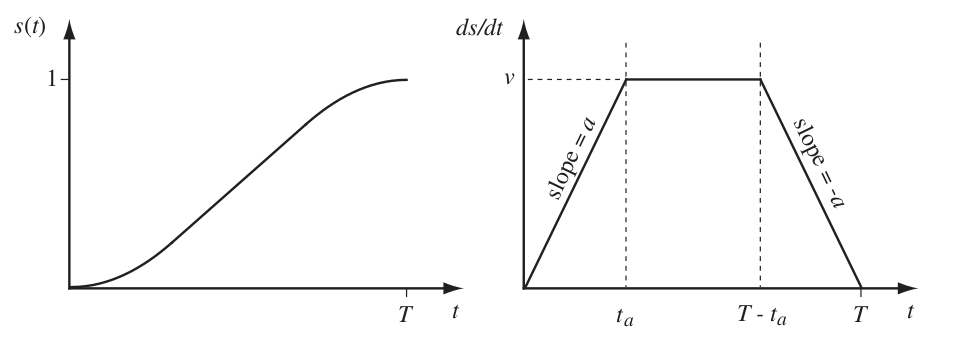
\includegraphics[width = 0.63\textwidth]{imagens/trapezoidal}
  \caption{Deslocamento e velocidade durante um deslocamento com perfil de velocidades trapezoidal. Tal perfil foi adotado neste trabalho.}
  \source{\citet{lynch2017modern}}
  \label{fig:trap}
\end{figure}

%% CONTROLE:
\subsection{Controle}

SUBSECTION EM CONSTRUÇÃO

Diversas abordagens podem ser utilizadas para a implantação de controladores em robôs omnidirecionais. Se pode realizar o controle das coordenadas desejadas, em x, y e z, ou o controle da posição de cada roda, independentemente. No caso, foram realizados três controladores de posição, em X, Y e $\omega$, utilizando a odometria discutida acima. O controlador então decide o set point de velocidade para cada roda, e envia os sinais de comando para um conjunto secundário de controladores de velocidade, 1 para cada roda. Se pode ver um esquema do sistema utilzado na FIgura \ref{fig:controle}.

\begin{figure}[h]
  \centering
  
\includegraphics[width = 0.45\textwidth]{imagens/edc}
  \caption{Arquitetura de controle utilizada.}
  %\source{\citet{lynch2017modern}}
  \label{fig:controle}
\end{figure}

Estabilidade, tipo do controle, proporcional, integral, derivativo, digital, tempo de ciclo, q q eu digo aqui, pô?

\citet{lynch2017modern}:

Loop de velocidade dentro do loop de posição. Posição das rodas ou posição em x e y e $\omega_z$?



\citet{rojas2006holonomic}: Sugerem que utilizar um controlador para cada roda é melhor do que para cada grau de liberdade. No nosso caso, é tranquilo pois temos apenas 3 rodas, mantendo o mesmo número de controladores. Devido à realimentação externa lenta, utilizam um preditor no robô. Não entram em detalhes.
motores:
https://www.banggood.com/6V-210RPM-Encoder-Motor-DC-Gear-Motor-with-Mounting-Bracket-and-Wheel-p-1044064.html?p=970719369296201312SG

Given a desired trajectory q d (t), we can adopt the feedforward plus proportional feedback linear controller (11.1) of Chapter 11 to track the trajectory: \cite{lynch2017modern}

\cite{samani2007comprehensive}: Definir os coeficientes dos PIDs é uma novela, pois devemos levar em consideração parâmetros que possuem muita variação, como o coeficiente de atrito do solo, características das baterias, entre outros. Controle deles é bem legal.
%q̇ com (t) = q̇ d (t) + K p ( q̇ d (t) − q(t)),
%(13.11)
%where K p ∈ R 3×3 is positive definite and q(t) is an estimate of the actual con-
%figuration derived from sensors. Then q̇ com (t) can be converted to commanded
%wheel driving velocities u com (t) using Equation (13.7).


%: seguimento de trajetória: malha aberta (3.6.1); Feedback (3.6.2) do livro: It is very similar to the controllers presented in [39, 100]. Others can be found in [8, 52, 53, 137]. Controle com uma matriz de ganhos K para o espaço de estados. Estável e tal. Comentam sobre camadas: planejamento -> decisão -> controlador em tempo real -> hardware.

\subsection{Limitações de Velocidade}

É importante ressaltar que toda a cinemática desenvolvida nas subseções anteriores não considera limites de velocidade para os atuadores. Numa aplicação real, entretanto, existe um ponto de saturação no acionamento de cada motor, que deve ser levada em consideração. Na Figura \ref{fig:twist_sat} se pode ver o efeito dessas limitações, conforme descrito em \citet{lynch2017modern}.

\begin{figure}[h]
  \centering
  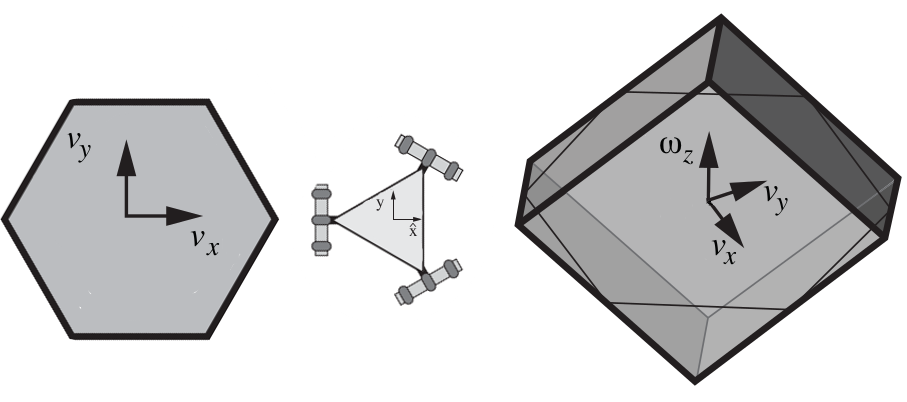
\includegraphics[width = 0.63\textwidth]{imagens/twist_sat}
  \caption{Limites de velocidade translacional e rotacional em função dos limites de saturação dos motores reais.}
  \source{Adaptado de \citet{lynch2017modern} para as coordenadas utilizadas.}
  \label{fig:twist_sat}
\end{figure}

Quando não há rotações ($\omega_z = 0$), o limite de velocidade do corpo do robô é descrito pelo hexágono mostrado na porção esquerda da Figura \ref{fig:twist_sat}: a maior velocidade possível é na direção em que uma das rodas está sendo ``arrastada'', e as componentes de velocidade das outras rodas se somam. Numa situação em que haja necessidade de rotação, a velocidade angular do robô se torna limitada da maneira mostrada no volume tridimensional à direita da Figura \ref{fig:twist_sat}, e se torna fácil enxergar que, para realizar um movimento de rotação na maior velocidade ângular possível, não se pode ter movimentos de translação, para que todos os componentes de velocidade das rodas contribuam apenas para a rotação.

Se pode dizer, então, que para aplicações reais nas quais a holonomicidade da plataforma é de fato desejável, se deve implantar um sistema de planejamento de trajetória que leve em consideração as limitações de velocidade descritas acima.

\section{Implementação dos algoritmos}
\label{sec:software}

SEÇÃO EM CONSTRUÇÃO

A implementação é difícil de encontrar nos trabalhos da bibliografia, portanto alguma coisa.

PROBLEMA: velocidade das rodas precisa o suficiente! Fazer experimentos em relação a isso.

ordem das coisas: \\
-análise dos códigos de cinemática \\
-desmembramento das funções do ritter \\
-código de acionamento dos motores \\
-bilbioteca orientada a objetos para o acionamento de cada motor e modularização do código\\
-controle de velocidade\\

Se implementou um controle proporcional simples, COLOCAR A LEI AQUI, mas se ontou que em trajetórias que necessitam do movimento das trê rodas em velocidades muito distintas se tem problemas. Para se mover em uma reta no eixo x, por exemplo, apenas as rodas 1 e 3 (verificar numeros) precisam girar, e na mesma velocidade, e fica simples de ver que o desempenho do controlador para as duas rodas vai ser similar. No entanto, na movimentação no eixo y são necessárias q a roda 1 esteja girando com o triplo da velocidade das outras duas (verificar), e assim vence a zona morta muito antes. Para solucionar isso, q q eu fáoc meu deus?\\
-implementação dos algoritmos de odometria \\
-testes para calibração dos movimentos (isso já é resultado??) \\
% 341.2/2pi pulsos/rad -> 54.3 pulsos/rad (0.01842 rad/pulso, 0.0029308323 rotações/pulso)
% VER O PAPEL NO MURAL

As equações implementadas relacionam as matrizes de transformação com a velocidade linear da periferia das rodas, $\dot{\phi}_i r$, em m/s. A leitura dos encoders é realizada em pulsos/$\mu$s. O fator de conversão aplicado é (em teoria) 534.18. Ao se utilizar o comando inverseKinematicsWorld, se obtêm as velocidades em m/s e a velocidade angular em rad/s. \\
-implementação do controle de posição \\
-algoritmo de limitação de velocidade, escalonamento \\
-organização do código \\
-interface com o usuário \\
-sequencia final de operação do código \\

O \textbf{Raspberry Pi} é um \emph{single board computer}, que utiliza a arquitetura \acrshort{arm} em seu processador, ideal para dispositivos alimentados por baterias por consumir pouca energia e gerar pouco calor. O processador possui quatro núcleos, e um \emph{clock} de 1,2 GHz -- poder computacional equivalente há um computador de mesa comum. O \acrshort{rpi} utiliza um sistema operacional GNU/Linux, e \emph{software} deve ser desenvolvido para ser executado nesta plataforma. Há ainda 40 pinos de \acrshort{gpio} que podem ser utilizados para conectar sensores, atuadores e diversos componentes, e suporte nativo a \acrshort{i2c} \citep{upton2014raspberry}.

O código de \citet{ritter2016modelagem} foi desmembrado em módulos, para separar a implementação já realizada da cinemática direta e inversa dos módulos de comunicação com o simulador utilizado. Foram escritos novos módulos para realizar a interface da Raspberry com os motores, sensores e periféricos em geral, e com essa modularidade se pode até fazer uma biblioteca para arduino blabalbalabballab, como na Figura \ref{fig:libs}.

\begin{figure}[h]
  \centering
  
\includegraphics[width = 0.45\textwidth]{imagens/edc}
  \caption{Bibliotecas utilizadas. TROCAR FIGURA}
  \label{fig:libs}
\end{figure}

Bibliotecas desenvolvidas: \\
- kinematics.h, a partir da cinemática de \cite{ritter2016modelagem}; \\
- rotary\_encoder.h, para realizar a decodificação dos encoders, desenvolvida por QUEM?? \cite{pigpio}, talvez?\\
- rpi\_interface.h, para realizar o acionamento e loops de controle para cada uma das rodas (desenvolvida pelo próprio autor);\\
- planning.h, que implementa as trajetórias de teste; \\
- user\_interface.h, que contem algumas funções básicas para conversar com o usuário, operador do sistema. IMAGINA Q MASSA UM APP C/ Bluetooth COM UM BOTÃO SÓ?

Todas as bibliotecas que utilizam entradas e saídas pelos pinos do RPi utilizam a biblioteca pigpio \citet{pigpio}, muito legalzona, até colocar nos agradecimentos.

Para calibrar o controlador em relação ao tamanho real das rodas, e obter velocidade ok, se utilizou a modelagem para definir qual deslocamento do robô, em rotação pura, necessita de 2pi rad de giro nas rodas. Foram feitos experimentos com diversos valors para calibrar isso ae.

Além de utilizar os comandos fornecidos por \citet{ritter2016modelagem}, foram implementados os modos de movimentação citados por \citet{loh2003mechatronics}: translação retilínea , translação curvilínea -- ambas sem alteração na orientação --, rotação pura e um caminho combinado de rotação em torno do seu centro e translação retilínia em relação às referências globais.

A obtenção do ângulo atual e m relação as coordenadas globais teve q ser diferente da utilizada por \citet{ritter2016modelagem}, que possuia um valor absoluto para este angulo. No caso do trablho descrito aqui, só se sabe a velocidade angular, que tambem deve ser integrada, e por isso podem aparecer mais erros.

O procedimento de opereação pode ser representado pelo diagrama apresentado na Figura \ref{fig:operation}.


\begin{figure}[h]
  \centering
  
\includegraphics[width = 0.45\textwidth]{imagens/edc}
  \caption{Fluxograma de operação do robô. TROCAR FIGURA}
  \label{fig:operation}
\end{figure}

%Para a comunicação dos periféricos com este computador, é necessário utilizar algum protocolo de comunicação. O protocolo \textbf{\acrlong{i2c}}, é geralmente utilizado em robôs, csom um grande suporte tanto pela \acrshort{rpi} (\cite{upton2014raspberry}) quanto pelos componentes em geral utilizados (\cite{MPU6050} e a bússola e o arduino se eu usar). Com este protocolo, descrito em \cite{semiconductors2000i2c}, dados podem ser transmitidos a 100 Kbps -- ou 400 Kbps quando utilizado o \emph{fast mode}. São utilizados duas linhas bidirecionais no barramento: SDA para os dados e SCL para os sinais de \emph{clock}. O número de dispositivos conectados ao barramento só depende do limite de capacitância descrito na especificação. Resistores de \emph{pull-up} são necessários para manter a linha em estado lógico alto quando não utilizada, porém estes resistores estão presentes internamente no \emph{Raspberry Pi}, por exemplo.

%O \emph{fast mode} é suportado pelo Raspberry Pi 3 B+.

Seguir o perfil de velocidade não é muito fácil, visto que dead zone. budibudibuidi \citet{indiveri2009swedish} trata saturação.

\section{Avaliação experimental}
\label{sec:experimental}

Se deseja avaliar o comportamento dos algoritmos implementados e da modelagem realizada operando o robô em três situações:
\begin{itemize}
  \item{trajetória retilínea, sem nenhum movimento de rotação, em diversas direções e com diversas velocidades de acionamento, conforme mostrado na Figura \ref{fig:reta};}
  \item{trajetória de rotação pura, analisando a variação de ângulo atingida em função do ângulo desejado e da velocidade desejada. Tal situação é ilustrada na Figura \ref{fig:giro};}
  \item{trajetória híbrida, realizando tanto uma translação retilínea arbitrária quanto uma rotação sobreposta, como no diagrama da Figura \ref{fig:hibrida}.}
\end{itemize}

\begin{figure}[h]
  \centering
  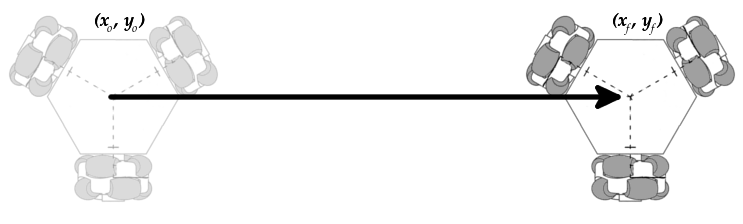
\includegraphics[width = 0.8\textwidth]{imagens/reta}
  \caption{Trajetória retilínea pura.}
  \label{fig:reta}
\end{figure}

\begin{figure}[h]
  \centering
  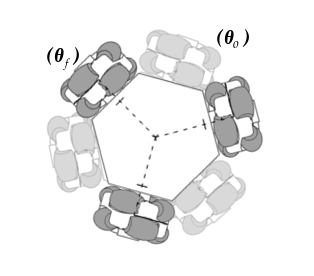
\includegraphics[width = 0.35\textwidth]{imagens/giro}
  \caption{Trajetória de giro.}
  \label{fig:giro}
\end{figure}

\begin{figure}[h]
  \centering
  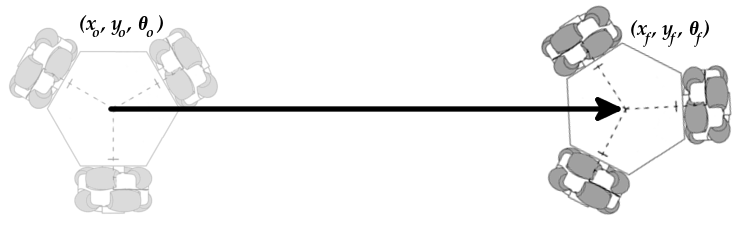
\includegraphics[width = 0.8\textwidth]{imagens/hibrida}
  \caption{Trajetória combinada.}
  \label{fig:hibrida}
\end{figure}

Se espera com a primeira trajetória, avaliar a robustez dos algoritmos quando se necessita o acionamento combinado de múltiplas rodas. Por exemplo, no eixo X, não há necessidade de movimento em uma das rodas. Em outras direções, se introduz movimentos mais lentos das rodas, o que já se viu que é um problema por causa do atrito viscoso da caixa de redução.

Com a trajetória de giro, em que as três rodas devem operar com a mesma velocidade, se deseja avaliar alguma coisa relacionada a isso. Na última trajetória, híbrida, se deseja mostrar o funcionamento do algoritmo de limitação de velocidade, e os efeitos deste fator.

Se notou que o acionamento dos motores depende de alguns fatores. Variando a frequência dos PWMs mudou o q?

O protótipo foi acionado sobre um papel enorme, com duas canetas de cores distintas instaladas nos orifícios destinados a tal.
